\documentclass{article}
\usepackage[dvipsnames]{xcolor}
\usepackage[paperwidth=20cm, paperheight=3.5cm, margin = 0cm, top=0.25cm]{geometry}
\usepackage{amsmath}


\usepackage{pgf}
\usepackage{tikz}
\usetikzlibrary{positioning, calc}
\usetikzlibrary{arrows,automata}

\tikzstyle{source}  = 
[
	draw,circle,fill=black,thick,inner sep=0mm,minimum size=2mm
]

\tikzstyle{box}  =
[
	draw,rectangle,thick,inner sep=2mm,
	minimum width=8mm, minimum height=8mm
]

\tikzstyle{redbox} = 
[
	draw,rectangle,thick,inner sep=2mm,
	minimum width=8mm, minimum height=8mm,
	fill=red, opacity=0.3, text opacity=1, draw opacity=1
]

\tikzstyle{bluebox} = 
[
	draw,rectangle,thick,inner sep=2mm,
	minimum width=8mm, minimum height=8mm,
	fill=blue, opacity=0.3, text opacity=1, draw opacity=1
]

\tikzstyle{lgreenbox} = 
[
	draw,rectangle,thick,inner sep=2mm,
	minimum width=8mm, minimum height=8mm,
	fill=SpringGreen
]

\tikzstyle{bluestate}  = 
[
	state, draw=blue, line width=2pt,
	fill=LimeGreen
]

\tikzstyle{redstate}  = 
[
	state, draw=red, line width=2pt,
	fill=LimeGreen
]

\tikzstyle{violetstate}  = 
[
	state, draw=Violet, line width=2pt,
	fill=LimeGreen
]



\renewcommand{\vec}[1]{\boldsymbol{#1}}

\begin{document}
\begin{center}
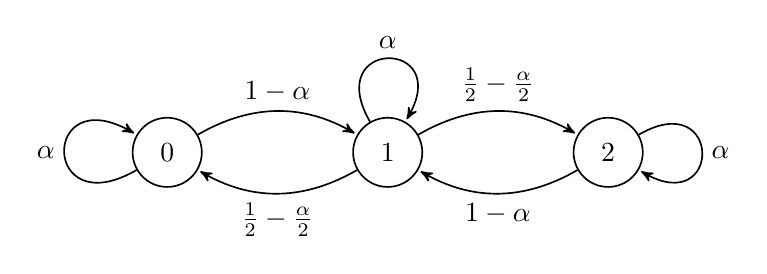
\begin{tikzpicture}[->,>=stealth',shorten >=1pt,auto,node distance=2.8cm,semithick]
                    
\node[state] (X0)               {$0$}; 
\node[state] (X1) [right of=X0] {$1$};
\node[state] (X2) [right of=X1] {$2$};

\path
	(X0) edge[bend left]  node[above]{$1-\alpha$} (X1)
	(X1) edge[bend left] node[below]{$\frac{1}{2}-\frac{\alpha}{2}$} (X0)
	(X1) edge[bend left]  node[above]{$\frac{1}{2}-\frac{\alpha}{2}$} (X2)
	(X2) edge[bend left] node[below]{$1-\alpha$} (X1)
	
	(X0) edge[in=150, out=210, looseness=7, loop, left]  node[left]{$\alpha$} (X0)
	(X1) edge[in=60, out=120, looseness=7]  node[above]{$\alpha$} (X1)
	(X2) edge[in=-30, out=30, looseness=7]  node[right]{$\alpha$} (X2);
\end{tikzpicture}
\end{center}

\end{document}
